\documentclass{beamer}
\usetheme{Berlin}  %% Themenwahl
\usecolortheme{beaver}

\usepackage{listings}
\usepackage{graphicx}
\usepackage{hyperref}
\usepackage[utf8]{inputenc}
\usepackage{amssymb}
\usepackage{amsmath}
\usepackage{esvect}
%\usepackage{mcode}
 
\title{Ray Tracing Optimization}
\author{Kashofer, Radschek, Wagner}
\date{\today}

%\section{Foliensection}
%\begin{frame} %%Eine Folie
%	\frametitle{Folientitel} %%Folientitel
%	Das ist eine Dummy-Section
%\end{frame}

\begin{document}
\maketitle
\frame{\tableofcontents[currentsection]}
 
\section{Profiling}
\begin{frame} %%Eine Folie
	\frametitle{Rendering time} %%Folientitel
  	\begin{itemize}
		\item original code: $45 \dfrac{sec}{Frame}$
		\item simple C-Code adaptions: $43 \dfrac{sec}{Frame}$
		\item replaced fix\_mul16 by ci\_mul looped functions: $36 \dfrac{sec}{Frame}$
		\item fix\_mul16 calls ci\_mul: $17 \dfrac{sec}{Frame}$
	\end{itemize}

\end{frame}

\begin{frame} %%Eine Folie
	\frametitle{Algorithm} %%Folientitel
  	\begin{figure}
		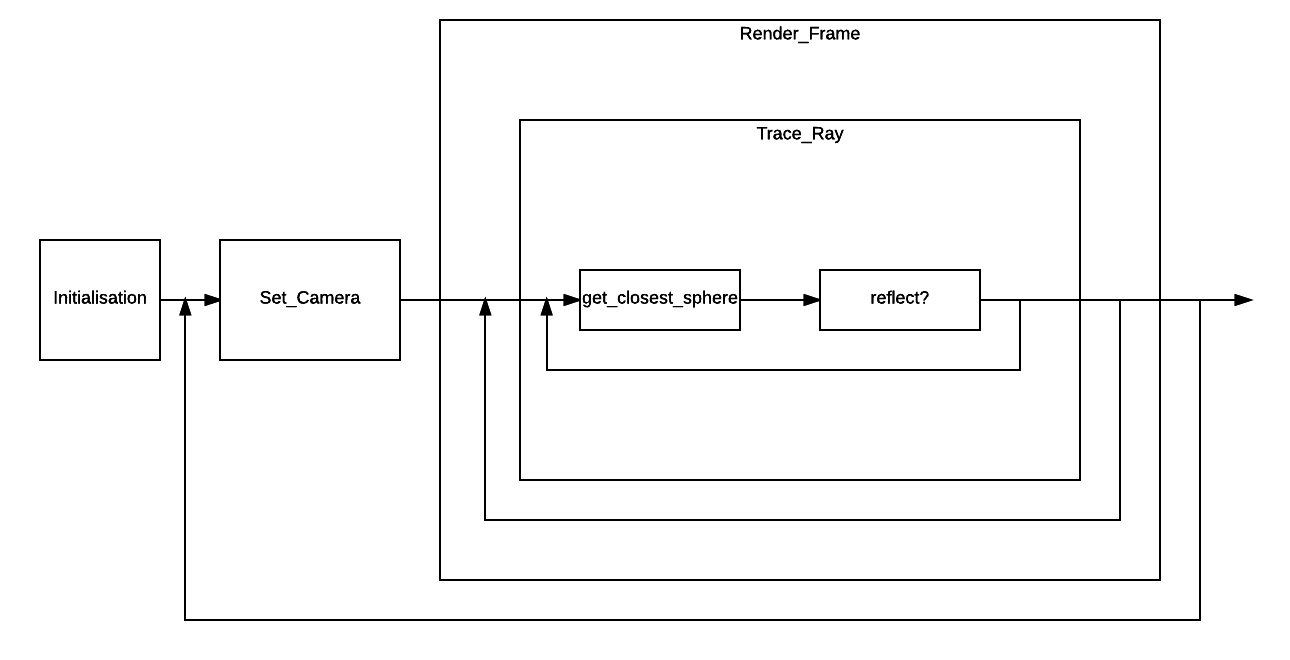
\includegraphics[width=\textwidth]{algo.png}
		\caption{Schematic of the algorithm}
	\label{fig1}
	\end{figure}
\end{frame}


\begin{frame} %%Eine Folie
	\frametitle{Functions} %%Folientitel
  	\begin{itemize}
		\item Initialisation: once in entire algorithm
		\item SetCamera: once every frame
		\item GetClosestSphere: up to REFLECT times per ray
		\item Reflect: up to REFLECT times per ray
	\end{itemize}
\end{frame}

\begin{frame} %%Eine Folie
	\frametitle{SW code structure} %%Folientitel
	getClosestSphere is a main function and contains a lot of loops\\
	$\quad$\\
	$\rightarrow$ Transition looped functions from SW to HW to achieve target speed
\end{frame}

\section{Optimization}

\begin{frame} %%Eine Folie
	\frametitle{HW ressources} %%Folientitel
	\begin{itemize}
		\item xyz Logic cells
		\item abc M9Ks
		\item uvw DSPs
	\end{itemize}
	$\quad$\\
	$\rightarrow$ Plenty Logic-cells (registers and LUTs), keep number of DSPs and M9Ks low
\end{frame}

\begin{frame} %%Eine Folie
	\frametitle{Main Idea}
	\begin{itemize}
	\item automate entire render-frame function in one pipeline
	\item use memory mapped interface
	\item set pipeline parameters (mostly the spheres) at initialisation
	\end{itemize}
\end{frame}
\begin{frame} %%Eine Folie
	\frametitle{Overview} %%Folientitel
		\begin{figure}[h]
		\centering
		\fbox{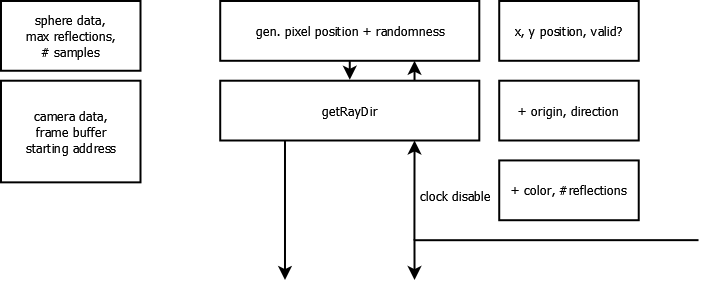
\includegraphics[width = 0.6\textwidth]{pics/frontend.png}}
		\caption{Pipepline 1}
	\end{figure}
\end{frame}
\begin{frame} %%Eine Folie
	\frametitle{Overview} %%Folientitel
	\begin{figure}[h]
		\centering
		\fbox{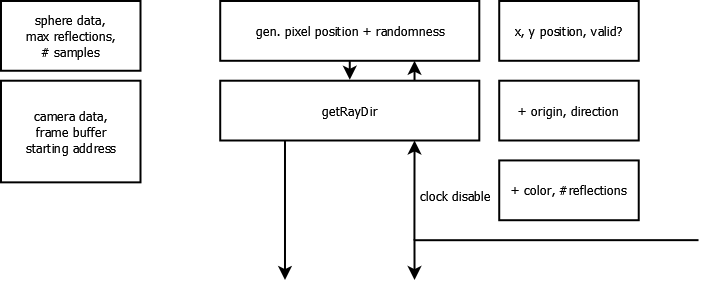
\includegraphics[width = 0.6\textwidth]{pics/frontend.png}}
		\caption{Pipepline 1}
	\end{figure}
\end{frame}
\begin{frame} %%Eine Folie
	\frametitle{Overview} %%Folientitel
	\begin{figure}[h]
		\centering
		\fbox{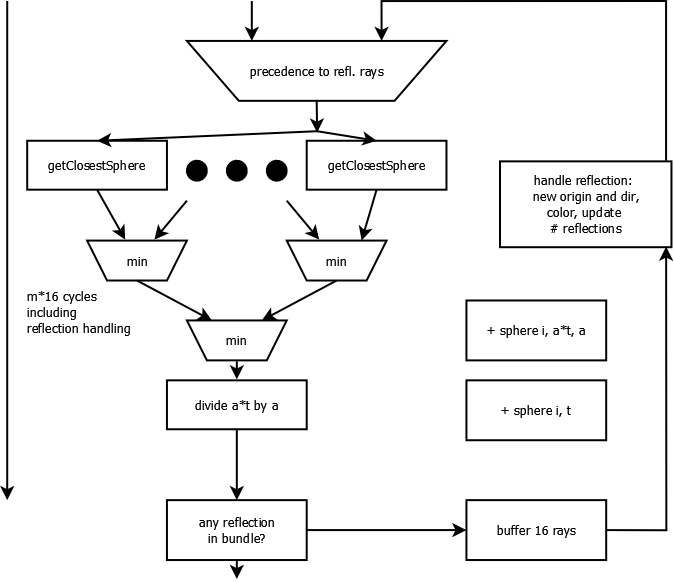
\includegraphics[width = 0.6\textwidth]{pics/middle.png}}
		\caption{Pipepline 2}
	\end{figure}
\end{frame}
\begin{frame} %%Eine Folie
	\frametitle{Overview} %%Folientitel
	\begin{figure}[h]
		\centering
		\fbox{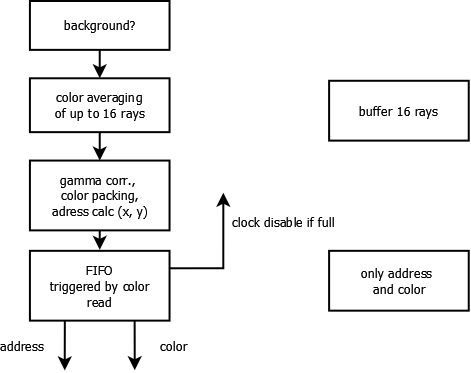
\includegraphics[width = 0.6\textwidth]{pics/backend.png}}
		\caption{Pipepline 3}
	\end{figure}
\end{frame}

\section{Usage}
\begin{frame} %%Eine Folie
	\frametitle{Calling the Pipeline} %%Folientitel
	\begin{itemize}
		\item Initialisation:\\
		each environment element has own address, write to it to update (no checks necessary)
		\item setCamera:\\
		each part of the camera has own address, write to it to update (read special address to see if write possible)
		\item startNewFrame:\\
		no special command necessary
	\end{itemize}
\end{frame}

\section{Evaluation}
\begin{frame}
	\frametitle{Resources (Pipeline 1)}
	\begin{itemize}
		\item \textbf{getPixelPosition}
			\begin{itemize}
				\item 2x random
				\item 2x add
				\item 10x 32 bit register (4 function, 6 overhead)
				\item 2x 16 bit register
				\item clock, enable, stall, reset, ...
			\end{itemize}
		\item \textbf{getRayDir}
			\begin{itemize}
				\item 6x multiplication
				\item 9x add/sub
				\item 51x 32 bit register (15 function, 36 overhead)
				\item clock, enable, stall, reset, ...
			\end{itemize}
		\item \textbf{additional overhead} (added after getRayDir)
			\begin{itemize}
				\item valid (1 bit)
				\item colour (3x 32 bit)
				\item reflections (3 bit)
			\end{itemize}
	\end{itemize}
\end{frame}

\begin{frame}
	\frametitle{Resources (Pipeline 2)}
	\begin{itemize}
		\item \textbf{getDistance}
			\begin{itemize}
				\item 8x add/sub
				\item 4x square function
				\item 4x multiplication
				\item 1x square root
				\item 50x 32 bit register
				\item 2x 16 bit register
				\item clock, enable, stall, reset, ...
			\end{itemize}
		\item \textbf{getClosestSphere}
			\begin{itemize}
				\item 8x getDistance
				\item 4x square function
				\item 2x add/sub
				\item 1 division
				\item 10x 32 bit register
				\item clock, enable, stall, reset, ...
			\end{itemize}
	\end{itemize}
\end{frame}

\begin{frame}
	\frametitle{Resources (Pipeline 2)}
	\begin{itemize}
		\item \textbf{additional overhead} (carried along each stage)
			\begin{itemize}
				\item valid (1 bit)
				\item colour (3x 32 bit)
				\item position (2x 32 bit)
				\item reflections (3 bit)
				\item origin (3x 32bit)
				\item denominator (a) (32 bit)
			\end{itemize}
	\end{itemize}
\end{frame}

\begin{frame}
	\frametitle{Resources (Pipeline 3)}
	\begin{itemize}
		\item \textbf{reflection (plus changing colour)}
			\begin{itemize}
				\item 11x add/sub
				\item 18x multiplication
				\item 1 comparator
				\item 500x 32 bit register
				\item clock, enable, stall, reset, ...
			\end{itemize}
	\end{itemize}
\end{frame}

\begin{frame}
	\frametitle{Timing}
	\begin{itemize}
		\item \textbf{getPixelPosition} 2 cycles
		\item \textbf{getRayDir} 4 cycles
		\item \textbf{getClosestSphere (without division)} 32 cycles
		\item \textbf{reflection (plus division n changing colour)} 50 cycles
		\item \textbf{padding to multiple of 16} 6 cycles
		\item \textbf{buffer rays of same pixel} 16 cycles
		\item \textbf{average pixel} 20 cycles
	\end{itemize}
\end{frame}


\end{document}